\documentclass[a4paper,twoside,12pt,nochapterprefix]{scrbook}

\usepackage{amsmath,amssymb,amsthm}
\usepackage[footnotesize,sl,SL,hang,tight]{subfigure}  % helpful package for aligning figures next to each other
\usepackage{multirow}
\usepackage{longtable} % tables over several pages
\usepackage[font={small,sl},hang,labelfont=bf]{caption} % configure captions
\usepackage{booktabs} % publication quality tables for LaTeX
\newcommand{\ra}[1]{\renewcommand{\arraystretch}{#1}}

%\ifpdfoutput{%
	\usepackage[pdftex]{graphicx}
	\usepackage[]{pdfpages} %for including full pdf pages
%}
\usepackage{rotating} % rotate figures

\usepackage[headinclude]{scrpage2}

% Font packages:
\usepackage{times}
\usepackage{helvet}   % sets sans serif font
\usepackage[T1]{fontenc}

%PDF hyperref config
%\ifpdfoutput{}

%\ifpdfoutput{}

\bibliographystyle{acmsiggraph}



% A4
%
\topmargin -0.5in
\textheight 9.3in
\textwidth 6.3in
\oddsidemargin 0.18in
\evensidemargin -0.22in
\parskip 0.1in
\parindent 0in

\renewcommand{\arraystretch}{1.5}
\renewcommand{\baselinestretch}{1}

% Stripped from acm siggraph bst and cls
\makeatletter

% no labels in bibliography.
\def\@biblabel#1{}

\newlength{\bibhang}
\setlength{\bibhang}{1em}

% Change in-bibliography biberence style
\def\thebibliography#1{%
  \section*{%
    \bibname\@mkboth{\sl\uppercase{\bibname}}{\sl\uppercase{\bibname}}}
  \list{\relax}{\setlength{\labelsep}{0em}
                \setlength{\itemindent}{-\bibhang}
                \setlength{\leftmargin}{\bibhang}}
  \def\newblock{\hskip .11em plus .33em minus .07em}
  \sloppy\clubpenalty4000\widowpenalty4000
  \sfcode`\.=1000\relax}

% Not sure what this does...
%\def\@citex[#1]#2{\if@filesw\immediate\write\@auxout{\string\citation{#2}}\fi
%  \def\@citea{}\@cite{\@for\@citeb:=#2\do
%    {\@citea\def\@citea{; }\@ifundefined
%      {b@\@citeb}{{\bf ?}\@warning
%      {Citation '\@citeb' on page \thepage \space undefined}}%
%{\csname b@\@citeb\endcsname}}}{#1}}

% Change in-document citation styles
\let\@internalcite\cite
\def\cite{\def\citename##1{##1}\@internalcite}
\def\shortcite{\def\citename##1{}\@internalcite}

\makeatother


\title{Scalable DOGs}
\author{Linus Wigger}

\begin{document}
\maketitle
{\centering \includegraphics*[width=0.5\textwidth]{../../../pics/initial_state}\\}

\chapter{Abstract}\label{sec:abstract}
% ----------------------------------------------------------------------------------------------
\chapter{Introduction}\label{sec:intro}\label{sec:prev_work}
%TODO make this into something
Developable surfaces, defined as smooth surfaces with zero Gaussian curvature, are locally isometric to a plane. They are of interest in areas like architecture or manufacturing because they can be obtained by transforming a plane via bending (but not stretching). As such, simulating developable surfaces is a TODO topic in computer graphics.\newline
This project uses the work from \cite{Rabinovich:DogNets:2018}, \cite{Rabinovich:DogShapeSpace:2018}, and \cite{Rabinovich:CurvedFolds:2019} as a starting point. These papers introduce the idea of using Discrete Orthogonal Geodesic nets (abbreviated as DOGs) to simulate deformations of developable surfaces.
 This approach has certain advantages compared to previous methods, mainly in terms of flexibility. They do not depend on predefined rulings, making it possible to explore the full shape space.\newline %TODO more and possibly correct
\cite{Rabinovich:DogNets:2018} made an editor where the user can interactively deform a DOG. Said editor supports creased folds (\cite{Rabinovich:CurvedFolds:2019}) and various types of constraints. The goal of this project was to work on the solver algorithm, mostly trying to make it suited for parallelization later on.\newline

% ----------------------------------------------------------------------------------------------
\chapter{Problem setting}\label{sec:problem}
%TODO \section{Terminology}?
%- dog with constraints given
The DOG is a quad mesh with many constraints. The mesh is initially constructed from a crease pattern - a two-dimensional set of curves defining the shape of the surface and its folds. Consequently, the set of crease curves can't be altered later (beyond changing the positions of the curve points).\newline
\begin{figure}
    \centering
    \setlength{\tabcolsep}{0.0130\linewidth}
    \includegraphics[width=0.8\linewidth]{../../../pics/0213_dog_from_creasepattern}
    \caption{Left: A crease pattern with one fold; Right: DOG obtained from the crease pattern with resolution $9$,$7$
      \label{fig:dog_from_creasepattern}}
\end{figure}
\begin{figure}
    \centering
    \setlength{\tabcolsep}{0.0130\linewidth}
    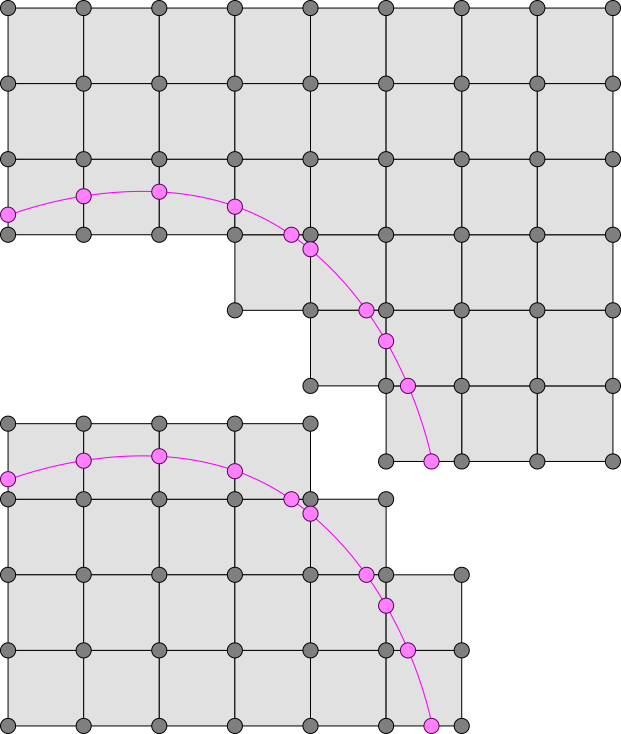
\includegraphics[width=0.33\linewidth]{../../../pics/0224_patches_split}
    \caption{Patches when separated from each other
      \label{fig:patches_split}}
\end{figure}
Figure \ref{fig:dog_from_creasepattern} shows an example of a crease pattern and the resulting mesh. The areas and vertices coloured in green are duplicated. All of the patches separated by the creases are actually disconnected, as seen in figure \ref{fig:patches_split}. They are held together by constraints on the curve points (which are shown in pink).\newline
%- objective to be minimized
\section{Objective function}\label{sec:objective}
The goal of the optimization is to minimize the bending energy of the DOG while satisfying all constraints. Most of the constraints are soft, meaning they are part of the objective function. The only constraints that are strictly enforced are the DOG constraints.
%TODO sums look ugly ... how to make a nice "set of constraints"?
\begin{equation}
f_{obj}(\mathbf{x}) = w_{bend} \cdot E_{bending}(\mathbf{x}) + \sum_{i \in \mbox{soft constraints}} w_i \cdot E_i(\mathbf{x})
\end{equation}
$\mathbf{x}$ in this case is a vector of size $3|V|$, containing the coordinates of all mesh vertices.\newline
%TODO bending energy ... which is |L(F0) - L(F)|^2, L being the Laplacian
The bending energy is computed by comparing the Laplacian $L$ of the current configuration to the Laplacian of the flat state
\begin{equation}
E_{bending}(\mathbf{x}) = |L(\mathbf{x_0}) - L(\mathbf{x})|^2
\end{equation}
Among the soft constraints, the following are the most important:\newline
The isometry constraints ensure that all edges in the mesh keep their original length. For each edge $e_i$, the squared difference between the current squared length $l_i^2$ and the correct squared length $l_{0i}^2$ is added to the objective. The weight associated with the isometry constraints should be rather high to ensure that almost no stretching happens. This is important because the allowed transformations for developable surfaces do not include stretching.
\begin{equation}
E_{isometry}(\mathbf{x}) = \sum_{i = 1}^{n_{edges}} (l_i^2((\mathbf{x})) - l_{0i}^2)^2
\end{equation}
Position constraints are the most common user-defined constraints. The user can select certain vertices to constrain, then drag them around so they have the desired positions. Each position constraint adds a simple spring energy to the objective. Assuming $P$ position constraints, each constraint having an associated vertex position $\mathbf{v}_i$ and target position $\mathbf{p}_i$, the energy from the position constraints can be written as:
\begin{equation}
E_{posconst}(\mathbf{x}) = \sum_{i = 1}^P (\mathbf{v}_i(\mathbf{x}) - \mathbf{p}_i) \cdot (\mathbf{v}_i(\mathbf{x}) - \mathbf{p}_i)
\end{equation}
%TODO edge point constraints
Similar to the position constraints are the edge point constraints. Their only difference is that they are defined on an edge point $\mathbf{e}$ instead of a mesh vertex $\mathbf{v}$. Edge points are defined by an edge $e \in E$ and a relative distance $t \in ]0,1[$. As such, the edge point constraints add the following term to the objective:
\begin{equation}
E_{edgepoints}(\mathbf{x}) = \sum_{i = 1}^R (\mathbf{e}_i(\mathbf{x}) - \mathbf{r}_i) \cdot (\mathbf{e}_i(\mathbf{x}) - \mathbf{r}_i)
\end{equation}
\begin{equation}
\mathbf{e_i} = t_i \mathbf{v}_{ai} + (1-t_i) \mathbf{v}_{bi}
\end{equation}
Where $R$ is the number of edge point constraints and the $r_i$ are the target positions. It should be noted that the users can't define edge point constraints directly, but they are still used sometimes.\newline
%The stitching constraints resemble the position constraints, but have two differences. First, the target location is not fixed: Two points should have equal positions. Second, the points in question are not mesh vertices but edge points, defined as a convex combination of two vertices. They are defined on the crease points - intersections of crease curves and mesh edges.
The stitching constraints have a very important role. They ensure that the different patches of the DOG are actually connected to each other. The way they are implemented resembles the edge point constraints. Instead of moving an edge point to a specific location, they hold two different edge points together.
\begin{equation}
E_{stitching}(\mathbf{x}) = \sum_{i = 1}^C (\mathbf{c}_{ai}(\mathbf{x}) - \mathbf{c}_{bi}(\mathbf{x})) \cdot (\mathbf{c}_{ai}(\mathbf{x}) - \mathbf{c}_{bi}(\mathbf{x}))
\end{equation}
The stitching constraints are generated automatically and can't be changed by the user (except for their weight). The stitching constraints are applied on all $C$ crease points, which are the points where the crease curves intersect the mesh edges. They come in pairs $\mathbf{c}_{ai}$ nad $\mathbf{c}_{bi}$, corresponding to duplicate edge points in two different patches.\newline
Angle constraints can also be defined on crease points. The solver will then attempt to make the folding angle at that location equal to the desired angle. The angle between the edges involved is not actually the same as the folding angle (which uses the surface tangents). This means that the correct angle $alpha_i$ between edges from different patches needs to be computed when the constraint is created. The objective works with the cosine of the angles, making angles with absolute value greater than $\frac{\pi}{2}$ problematic. The energy for $A$ angle constraints between edges $e_{ai}$ and $e_{bi}$ from different patches is computed as:
\begin{equation}
E_{angleconst}(\mathbf{x}) = \sum_{i = 1}^A (\cos( \angle(e_{ai}, e_{bi})(\mathbf{x})) - \cos(\alpha_i ))^2
\end{equation}
There are still more parts of the objective function. Some are variants of the elements above (e.g. paired vertices), others are rarely relevant and have more complicated formulas. They will not be described in more detail.\newline
%- details on optimization
\section{Optimization}
The optimization is formulated as a Sequential Quadratic Programming problem and solved using the PARDISO (TODO src) solver. Each iteration starts by updating all constraints. Following that, PARDISO computes a better solution for the current constraints.
% ----------------------------------------------------------------------------------------------
\chapter{ADMM}\label{sec:admm}
As can be seen in the previous chapter, most parts of the objective function are separable in the sense that they can be split into contributions from different patches. This is the case for the bending energy, isometry constraints, and position constraints. The stitching and angle constraints connect vertices across patch boundaries and are therefore not separable.\newline
The idea is to use the alternating direction method of multipliers (ADMM) as described in [TODO citation]. This method can be applied to a problem of the form
\begin{equation}
\begin{array}{lr}
\mbox{min} & \Sigma_{i=1}^{N} f_i(\mathbf{x}_i) \\
\mbox{s.t.} & \Sigma_{i=1}^{N} A_i \mathbf{x}_i = c
\end{array}
\end{equation}
In this case, the $\mathbf{x}_i$ are the coordinate vectors for each patch and the stitching constraints match the second line.\newline
\section{Variant: Subsolvers}
The most basic ADMM-like method optimizes each patch separately. The stitching constraints on the global mesh are replaced by edge point constraints on the patches. After each iteration, these edge point constraints get updated with the positions obtained in the adjacent patches. This method requires no additional objective terms.\newline
\section{Variant: Variable Splitting ADMM}
Variable Splitting ADMM (TODO see algorithm 1 in src) works similar to Subsolvers but adds a few extra elements: The local objective functions% $f_{obj}^i(\mathbf{x})$
 are extended by an additional term $\frac{\rho}{2}|A_i - z^{k+1}_i -\frac{\lambda_i^k}{\rho} |^2$. $lambda$ and $z_i$ are other extra variables that are updated in each iteration. The $z_i$ are set to $A_i x_i - \frac{1}{N}\sum_{j=1}^N(A_j x_j + \frac{\lambda_j}{\rho})$. After obtaining a new $x_i$ from the solver, the $\lambda_i$ get updated to $\lambda_i - \rho(A_i x_i - z_i +\frac{\lambda_i}{\rho})$
\section{Variant: Proximal Jacobian ADMM}
Proximal Jacobian ADMM (TODO see algorithm 4 in src) adds another extra term to VSADMM and changes the way $z_i$ and $\lambda$ are computed. A proximal term $\frac{\rho}{2} dx_i^T P dx_i$ is added, where $dx_i$ is the difference $x_i - x_0i$ ($x_0i$ being the resulting $x_i$ from the previous iteration) and $P$ is a diagonal matrix. $z_i$ in this variant is computed as $A_i x_i - \sum_{j=1}^N + \frac{\lambda}{\rho}$ and $\lambda$ (which is constant across patches) becomes $\lambda - \rho \gamma \sum_{i=1}^N A_i x_i$ ($\gamma$ being a damping parameter > 0).
\section{ADMM results}

%TODO the ADMM methods are crap
% - Subsolvers is just horribly slow
% - VSADMM and Prox-JADMM have stability issues
The ADMM methods are not good for this problem. All of them are extremely slow at moving away from the initial state. Figure \ref{fig:admm_results} plots the objective function for a simple problem over $1000$ iterations. Even ignoring the exact numbers (because all methods have slightly different objective functions) the existing "standard" solver reaches a solution very quickly (less than $50$ iterations after which the solution stays constant). The other methods are slow at best and at worst there are stability issues: Proximal Jacobian ADMM can spontaneously break everything, even long after it looks like the DOG has stabilized.\newline
\begin{figure}
	%TODO add an image of what's happening: folded initial state -> flatten
    \centering
    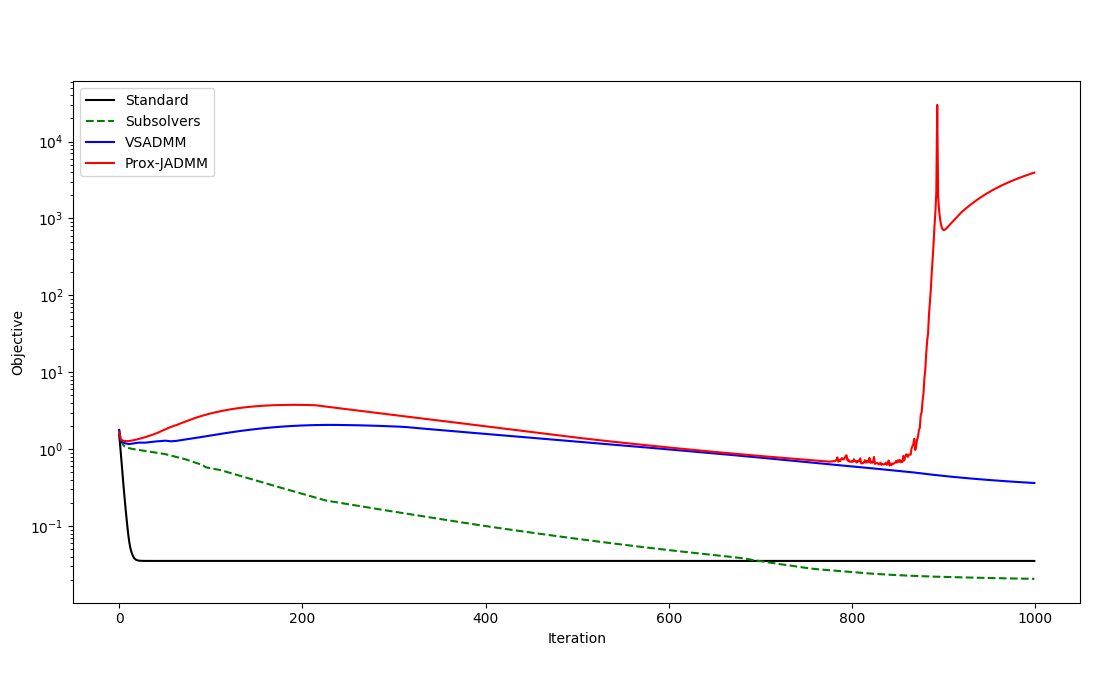
\includegraphics[width=0.99\linewidth]{../../../pics/0221_flattenplot_from_1025}
    \caption{Objective function values for flattening a simple DOG}
    \label{fig:admm_results}
\end{figure}
Angle constraints are difficult to enforce in the ADMM solver because, like the stitching constraints, they connect vertices from different patches to each other. Updating the coordinates of points outside the local patch after each iteration causes heavy jittering in the results (due to overshooting from both sides). Angle constraints could in theory be reformulated to work with a crease curve of the DOG instead of arbitrary edges. This would allow them to be split into two half-constraints that use only local information on each patch.\newline
The main problem with the ADMM variants is that they assume the crease curves to be constant. Given that finding the shape of the curves in 3D is one of the more important aspects of the optimization, this is a very bad assumption. Additionally, ADMM as described in TODOsource assumes that the problem  is convex, which it is not (due to all the constraints).\newline

% ----------------------------------------------------------------------------------------------
\chapter{Coarse method}\label{sec:coarse}
It's very important to know where in 3D the crease curves end up but the ADMM methods are unsuited for that. An approach that can handle deformations of the curves was needed.\newline
The idea behind the following method is to quickly compute a guess for the crease curves in 3D and use these to optimize all patches locally. To compute the guess, a coarse version of the global DOG will be used.\newline
In the spirit of multigrid methods, a single iteration with the coarse mesh works in four main steps:\newline%solve coarse globally; coarse-to-fine update; solve fine locally; fine-to-coarse update
\begin{itemize}
\item Coarse solve
\item Coarse-to-fine update
\item Fine solve
\item Fine-to-coarse update
\end{itemize}
%TODO pseudocode?
The coarse solve is a standard global solver iteration. It is fast because it doesn't use the actual DOG but a coarse version of it. The fine solve consists of solving each patch separately (like in ADMM). The coarse-to-fine and fine-to-coarse updates transfer information between the two resolutions.\newline
How exactly the four steps work varies slightly between most of the tried variants. The coarse and fine solves work the same for the most part, plus or minus a few constraints. The coarse-to-fine and especially fine-to-coarse updates can differ very much. It is like that because for DOGs there is no straightforward way to coarsen/subdivide a mesh while fulfilling all necessary constraints.\newline
The coarse-to-fine update always involves the crease curves. The crease points from the coarse mesh get used as constraints in the appropriate fine patches. For some points on the fine curve this involves interpolating between coarse curve points
\section{Coarse mesh}\label{sec:coarse_construction}
The coarse mesh gets constructed using the same method as the fine one, the only difference being its resolution, which is half the regular resolution in both $x$ and $y$, rounded up. As the resolution corresponds to the number of vertices in each direction, this ensures that each coarse edge consists of two fine edges and each coarse quad covers four fine quads (when looking at a flat DOG).\newline
Given the fine and coarse meshes, an auxiliary data structure that links the two gets constructed. This data structure holds all information necessary to switch between resolutions. Important parts include the fine-to-coarse and coarse-to-fine arrays. For each vertex in the fine and coarse mesh, they store the index of the vertex that has the same position in the other resolution. Given that the fine mesh is roughly four times the size of the coarse mesh, there are of course many vertices with no direct counterpart. For those, the arrays store a negative number which can further identify the type of the vertex in question.\newline
\begin{figure}
    \centering
    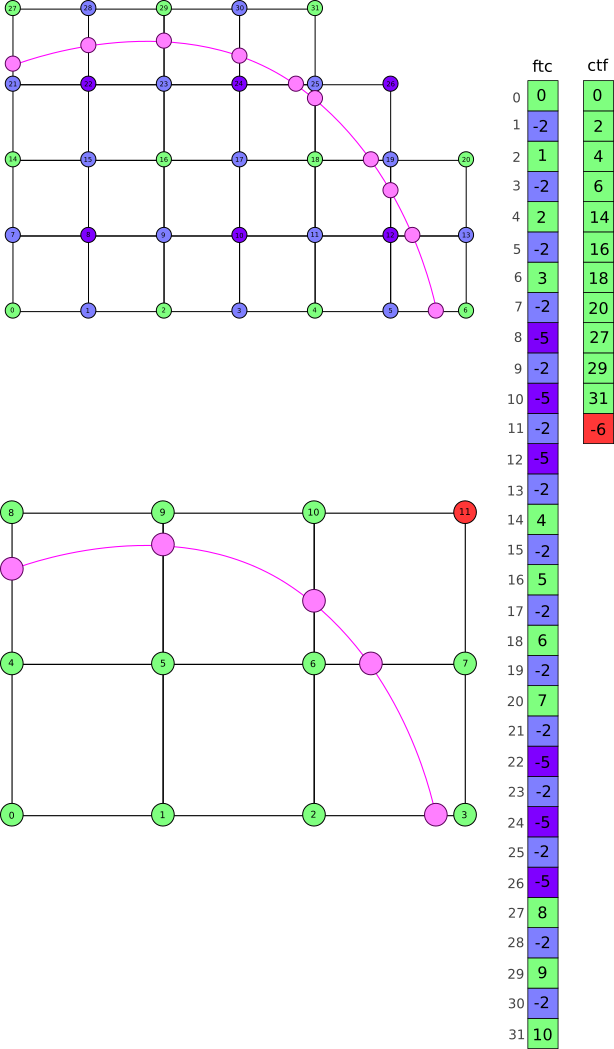
\includegraphics[width=0.6\linewidth]{../../../pics/0213_ftc_ctf}
    \caption{Top: Fine patch; Bottom: Coarse patch; Right: Fine-to-coarse and coarse-to-fine arrays
      \label{fig:ftc_ctf}}
\end{figure}
Figure \ref{fig:ftc_ctf} shows an example of a small patch, its coarse version, and the associated helper arrays. The type of a vertex determines its colour:\newline
\begin{itemize}
\item \textbf{Link} vertices are those that are part of both meshes. They are coloured green in the picture.
\item \textbf{Fine-only} vertices appear only in the fine mesh. They can further be differentiated into
\begin{itemize}
\item \textbf{I}-vertices (shown in light blue) which are adjacent to at least one link vertex
\item \textbf{X}-vertices (shown in purple) whose only direct neighbours are other fine-only vertices
\end{itemize}
\item \textbf{Coarse-only} vertices (red in the picture) can only appear near the creases. As their name implies, they exist only on the coarse mesh.
\end{itemize}
\section{FineCoarseConversion}\label{sec:conversion}
This section provides a detailed description of the data structure linking the fine and coarse meshes. It is initially constructed after the meshes were created from the crease pattern and exploits the fact that all vertices lie in the $xy$-plane at that moment.\newline
At the beginning, finding the link vertices is the most important step. The most basic way to identify the link vertices is to compare the coordinates of vertices in the fine mesh with those in the coarse mesh, but this is a brute force approach that is very expensive for large meshes.\newline
%TODO more
Originally the method to find equivalent vertices in the fine and coarse meshes was a flooding algorithm. It started at one vertex and traversed the meshes in a BFS manner. This was quite error-prone and required quite a bit extra work to find a good origin and cross from one patch to another.\newline
%TODO picture and/or formulas
The flooding method was replaced by another algorithm which treats each patch separately. Using the bounding box of all vertices whithin each patch and the distance between adjacent vertices it creates two rectangular grids per patch (one for the fine patch and one for the coarse patch). Each mesh vertex is assigned to one position in a grid. The advantage here is that it is very easy to go from fine to coarse and vice versa. As an example, the vertex at coarse grid coordinates $(1,2)$ corresponds to the vertex at fine grid coordinates $(2,4)$, the vertex at coarse coordinates $(1,3)$ is linked to the vertex at fine coordinates $(2,6)$, and the vertex at fine coordinates $(2,5)$ is a fine-only I-vertex that lies between them.\newline
In the end, this data structure holds all information that might be needed when changing between the fine and the coarse DOG. Most often it is used to convert indices of link vertices from one resolution to the other. It can also be used to determine the type of a vertex, map fine-only vertices to coarse edges or quads, and assign crease points in the two resolutions to each other.\newline
\section{Constraints on the coarse mesh}\label{sec:coarse_constraints}
The coarse mesh should provide good approximation of the fine solution. This means subjecting it to the same constraints as the fine mesh. For some constraints this is easier than for others.\newline
The main DOG constraints of equal angles between edges around one vertex still apply, just using the topology of the coarse mesh now. Similarly, isometry and stitching constraints work like in the fine mesh but using other vertices.\newline
The user-defined position and angle constraints can cause issues. If a constraint is defined on a fine-only vertex, then the coarse solver would need to approximate that constraint. This wasn't implemented, so all user-defined position constraints need to use link vertices.\newline
%TODO image of relevant fine and coarse vertices?
As the angle constraints lie on edge points (i.e. between two mesh vertices) it is impossible to have all relevant vertices be link vertices. The constraint is thus modified a bit: Assuming one of the vertices involved is a link vertex, then the other is a fine-only I-vertex. In the coarse mesh, the I-vertex gets replaced by the next coarse vertex in that direction. The coarse vertex in question can be found quickly if a mapping from I-vertices to coarse edges is precomputed.\newline
\begin{figure}
    \centering
    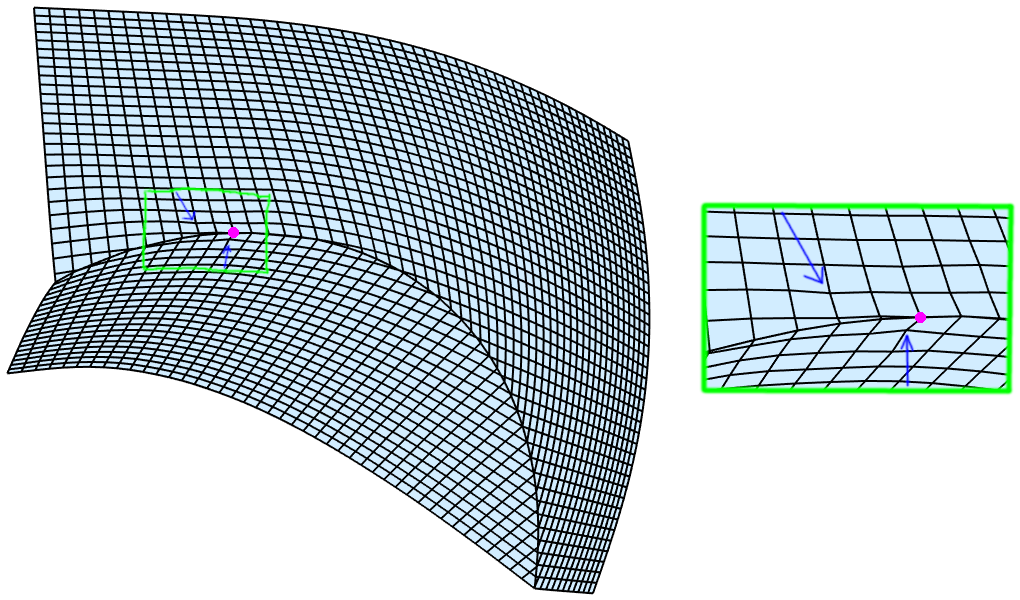
\includegraphics[width=0.9\linewidth]{../../../pics/0308_angleconstraint_ugliness}
    \caption{Angle constraint at the pink marker. On the right is zoomed-in view of the green rectangle. Blue arrows point to vertices that lie outside the local plane.}
      \label{fig:angleconstraint_ugliness}
\end{figure}
The coarse angle constraints definitely change the results of the computation, but arguably it is an improvement. Angle constraints often result in shapes like in figure \ref{fig:angleconstraint_ugliness}, where the angle constraint is technically satisfied at the crease point, but the mesh doesn't look smooth in that region. Taking a coarse angle constraint lessens this local irregularity.\newline

\section{First coarse solver}\label{sec:first_coarse}
The first serious variant of the coarse method starts with a global solver iteration on the DOG described in the previous section.\newline
In the coarse-to-fine update, only the crease points are relevant. Interpolating between the coarse curve points results in coordinates for the fine curve points. These are used as edge point constraints and replace the stitching constraints on the patches.\newline
The fine-to-coarse update is almost nonexistent in this variant. Assuming that any position constraints lie on link vertices, their target positions are equivalent in both coarse and fine.\newline
\section{Fine-to-coarse update}\label{ftc_update}
Finding a good way to update the coarse mesh after the fine patches are done is quite difficult. The most straightforward approach would be to take the coordinates from the fine mesh and assign them to the appropriate vertices in the coarse mesh. This does not work for coarse-only vertices, so those need to be handled in another way.\newline
The first coarse solver lacked a fine-to-coarse update and was not too bad, so it's not unthinkable that the fine-to-coarse update could just ignore the coarse-only vertices. That said, it is not a good idea to only update some parts of the coarse mesh while leaving others as they were.\newline
% Two more methods: no coarseonly, curve submeshes ... have their own sections
The following two sections (\ref{sec:coarse_construction_alt} and \ref{sec:curve_submeshes}) concern major changes made to remove the coarse-only vertices. The remainder of this section is dedicated to variants that do try to update the coarse-only vertices while keeping the existing meshes.\newline%
% silly extrapolation
Finding a good way to update coarse-only vertices requires knowing some facts about them. Coarse-only vertices appear only on the boundary of a patch, near creases. They are always outside the "real" patch, on the other side of a curve compared to the majority of all vertices in the patch. The idea is to use information from assorted close-by fine vertices to compute coordinates for each coarse-only vertex.\newline
\begin{figure}
    \centering
%    \setlength{\tabcolsep}{0.0130\linewidth}
%	\includegraphics[width=0.8\linewidth]{../../../pics/whatever}
    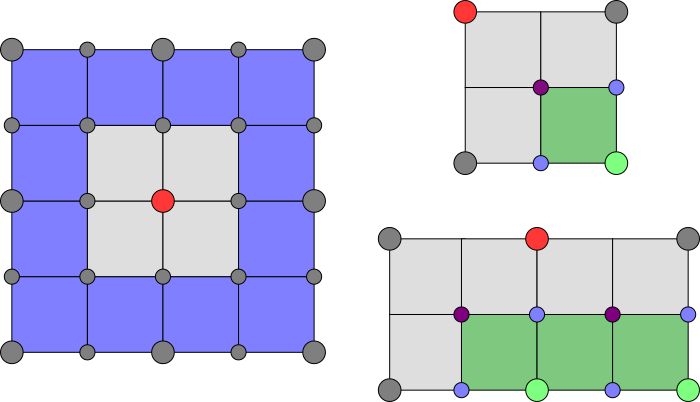
\includegraphics[width=0.75\linewidth]{../../../pics/0221_nearby_fine_quads}
    \caption{Left: Potential fine quads near a coarse-only vertex; Top right: Minimum of one nearby quad; Bottom right: Realistic case with three nearby quads
      \label{fig:coarseonly_neighbourhood}}
\end{figure}
Each coarse-only vertex can potentially have any of the blue quads shown in figure \ref{fig:coarseonly_neighbourhood} nearby, but only one of them is guaranteed to exist. The four quads in the middle are never present (because if any of them were, the central vertex wouldn't be coarse-only). Realistically, there will never be a full ring around a coarse-only vertex and testing showed that the number of fine quads near a coarse-only vertex is usually between $1$ and $6$.\newline
Multiple methods using the nearby fine quads to extrapolate coordinates for the coarse-only vertex were implemented and tested, but none of them were particularly good and most had serious stability problems. As it happens, the whole plan was fundamentally flawed: The fine result may satisfy all necessary constraints on the fine DOG, but directly inserting some of those coordinates into the coarse mesh will generally not satisfy the coarse DOG constraints.\newline
% soft constraints
Instead of directly setting the coordinates to be equivalent, adding another set of soft constraints turned out to be a solution of sorts. Each link vertex in both resolutions gets an extra position constraint moving it to its equivalent in the other resolution. These link constraints have a much lower weight than actual position constraints, so they can keep the fine and coarse meshes in similar shapes, but not to the detriment of any important constraints.\newline
%There are two glaring flaws with this: First, the coarse-only vertices do not get updated this way. Second, the fine coordinates may satisfy the DOG constraints on the fine mesh, but inserting them into the coarse mesh generally doesn't satisfy the coarse DOG constraints.\newline
\section{Alternative coarse mesh construction}\label{sec:coarse_construction_alt}
To avoid having to update coarse-only vertices, one variant used a different strategy to obtain the coarse mesh. Instead of building it roughly the same way as the regular DOG, the coarse DOG is constructed by removing vertices from the fine mesh. By removing every second row and column of vertices and connecting the remaining vertices correctly, we get a coarser mesh where every vertex is a link vertex.\newline
The resulting coarse mesh no longer covers all fine patches. The most problematic part is what happens to the crease curves in the coarse mesh. Only a limited number of crease points are still in the coarse mesh and, crucially, the endpoints of the curve (i.e. where the crease curve intersects the mesh boundary) are not among them. This makes it impossible to interpolate coordinates for the crease points near the boundary.\newline
%TODO a picture ... shows the result of this: The mesh is clearly disconnected at the ends of of the crease. Attempts to fix this by adding some extra constraints produced no better results, and so this particular method was scrapped
\subsection{Results}
With the alternative coarse mesh construction, the endpoints of all crease curves and all crease points between the endpoints and the closest coarse crease point can't be interpolated from the coarse mesh. If nothing is done with those points, the results look like in figure \ref{fig:alt_coarse_result}. There is a clearly visible disconnect between the two patches at the boundary.\newline
\begin{figure}
    \centering
    \includegraphics{../../../pics/1218_unconstrained_curve_end}
    \includegraphics{../../../pics/1218_dislocated}
    \caption{Result when using the alternative coarse construction without any further constraints. The region near the curve end is problematic, especially if said region is larger like in the right mesh.}
      \label{fig:alt_coarse_result}
\end{figure}
It's possible to reconnect the boundary parts of the crease using edge point constraints. This leads back to the same problem that ADMM had: The crease points near the boundary assume that the curve shape is constant even though it isn't, and so those parts only change very slowly. By altering the associated weights at runtime, it's possible to get fast changes initially and connected patches later. It's still usually not worth it because one of the two problems almost always remains and the reweighting process would have to be automated for general user inputs.\newline


\section{Curve submeshes}\label{sec:curve_submeshes}
This variant was "invented" after realizing something: Most problems arise near the crease curves. Anything related to stitching, angle constrints, coarse-only vertices will only happen around a curve. The following idea came up: Create a new type of mesh that specifically handles these problematic areas.\newline
\begin{figure}
    \centering
    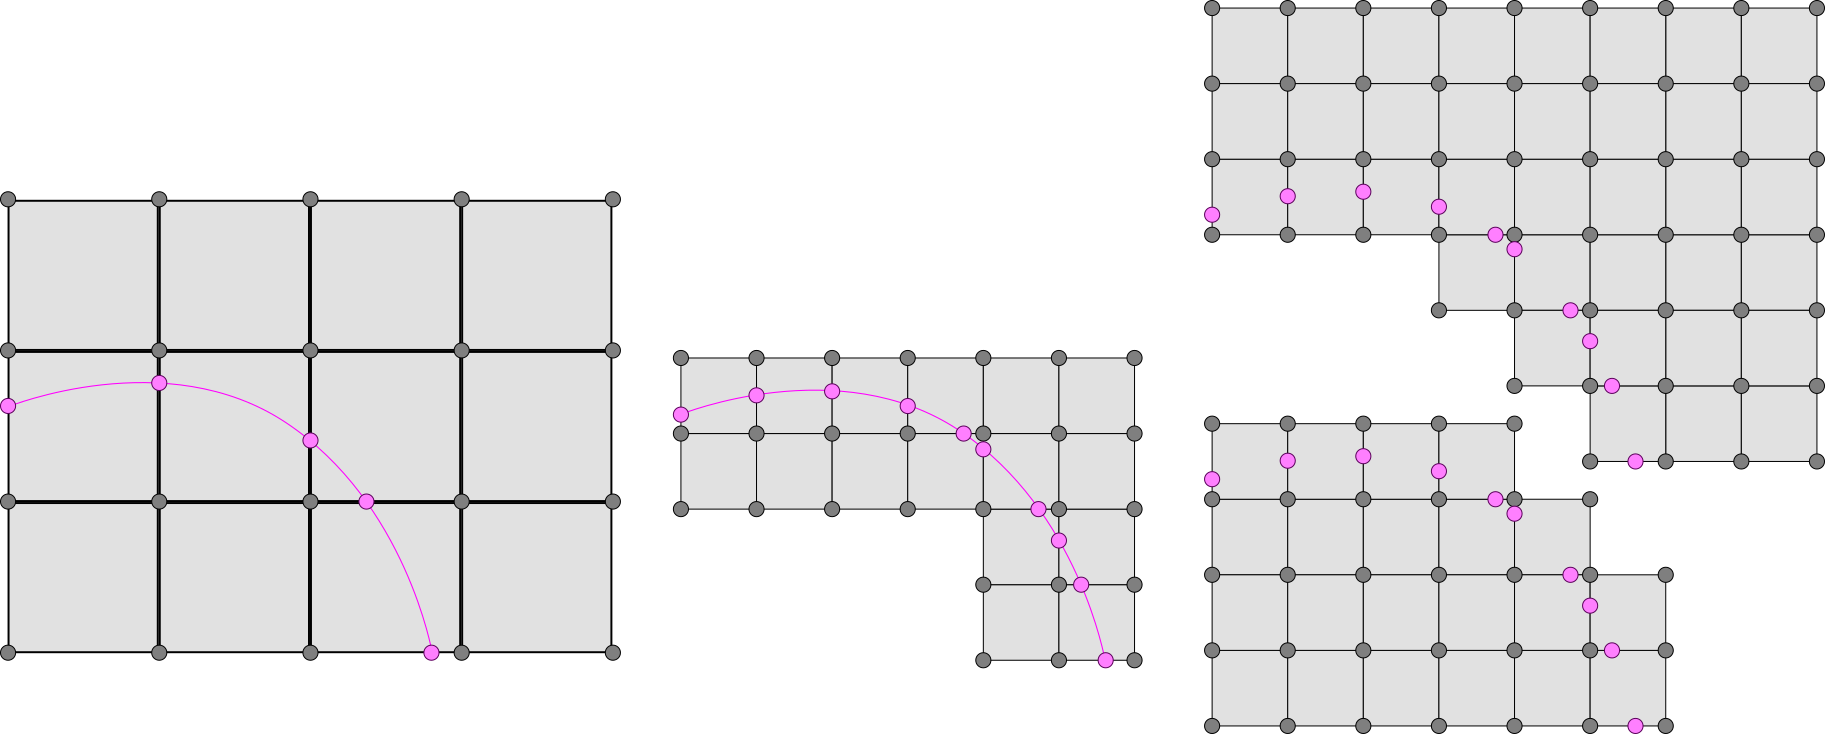
\includegraphics[width=0.99\linewidth]{../../../pics/0306_curvesubmesh}
    \caption{From left to right: Coarse mesh, curve submesh, patch submeshes}
      \label{fig:curve_submesh}
\end{figure}
As an addition to the entire coarse mesh and the fine patch submeshes, we introduce curve submeshes. These are fine meshes containing only the areas near a crease curve. This means that they contain vertices from multiple patches while still being very small (and thus fast to compute solutions). The curve submeshes function as interfaces between the coarse mesh and the fine patches. To that purpose, the curve submeshes contain fine versions of all coarse quads through which a curve passes. This includes fine vertices corresponding to the previously coarse-only-vertices. An example of the full set of meshes is displayed in figure \ref{fig:curve_submesh}. Note that all elements near the curve in both the coarse mesh and the curve submeshes are duplicated. They are also duplicated in the fine mesh, but the patches are already separated in the picture and so all duplicate elements are visible there.\newline
A single iteration with curve submeshes works as follows: Initially, the coarse solver produces guesses for certain points of the curves. The curve submeshes use those as constraints and compute the position of all crease points, while also ensuring that angle constraints are satisfied (remember, those are among the constraints that work across patch borders). The patches then gather the shape of their borders from the curve submeshes and work on minimizing their local objective functions. The curve submeshes also contain the necessary parts to propagate data back from fine to coarse.\newline
\subsection{Results}
The method using curve submeshes works reasonably well: The patches are connected at the creases. There are no bizarre deformations that break all constraints. Everything is fast enough to edit the constraints interactively. There are still two problems.\newline
As mentioned in section \ref{ftc_update}, updating the coarse vertices with coordinates from fine vertices is not a good idea. The curve submeshes may have fine versions of the coarse-only vertices, but the fine-to-coarse update still needs another method.\newline
Second, the results of the curve submesh solver are almost indistuingishable from those obtained by just using the coarse mesh and the fine patches. As there is no real point to introducing curve submeshes (and therefore more points failure) if they don't actually improve the result, the curve submeshes were scrapped.\newline
%There are many ways that the curve submeshes (section \ref{sec:curve_submeshes}) could still be useful. 
%\chapter{Parallelization}
% ----------------------------------------------------------------------------------------------
\chapter{Results}\label{sec:results}
%Figure \ref{fig:results_plotblock} shows results from multiple tests with varying crease patterns, resolution, and solver method. Figure \ref{fig:results_legend} and table \ref{tab:res_and_vnum} hold related information. Shown on the left side of figure \ref{fig:results_plotblock} is the initial state, with a final result on the right. It's actually the result from using the standard solver and the second-largest mesh.\newline
%What's happening: The mesh starts flat, then two positional constraints get added at the lower left and upper right corners. They are moved steadily over $250$ iterations before reaching their final positions (a dotted line marks iteration $250$ in each plot).\newline
%As can be seen, the different variants of the coarse method perform qualitatively similar to the standard solver. There are occasional hiccups (like in the top left example with link weight $0.01$), but usually the result looks almost the same, no matter the method. In all cases, the standard solver gets the lowest objective values, which isn't surprising, given that it just tries to minimize the objective directly. For the coarse method, it seems like the fine-to-coarse update via soft positional constraints on the link vertices is usually better than having no fine-to-coarse update.\newline
%As mentioned at figure \ref{fig:results_timeperiteration}, the time per iteration is averaged over iterations $10$ to $240$. Figure \ref{fig:results_cornerstime} shows how much time each iteration takes in an ordinary case. As can be seen, the time per iteration is roughly constant as long as the constraints are moving. The first few iterations often take longer, so they get left out of the average. After iteration $250$ (i.e. once the constraints are fixed) the solver tends to quickly reach a solution, whereupon the time per iteration drops dramatically, though not always: Especially if the mesh is larger, the convergence to a solution may take longer. In some cases, the standard solver actually becomes slower at the end. \newline
%In most cases, the standard and coarse solver lead to very similar results (as in figure \ref{fig:results_compare_valley}), but the crease pattern "parallel\_curves\_4" is one of the exceptions. As seen in figure \ref{fig:results_compare_curves}, the two solver modes have significantly different results.\newline
% In all examples the first few iterations are a bit rough (compared to how smooth the curves are afterwards). The process can be regarded as three phases: First the solver approaches some sort of "solution", which is often accompanied by a peak in the objective. In the second phase, the "solution" has been found, but the constraints are still changing. Once the constraints reach their final state, the DOG remains constant (though sometimes it ends up in a short loop that's not really visible).
\section{Test setup}
%- do it with 1curve, 4corners, valley, and parallelcurves4
%- different resolutions
%- standard, coarse with ftc 0 0.001 0.01 0.1 1
%- posconstraints at two corner points, moving over 250 iterations
%- store data for 300 iterations
\begin{figure}
    \centering
    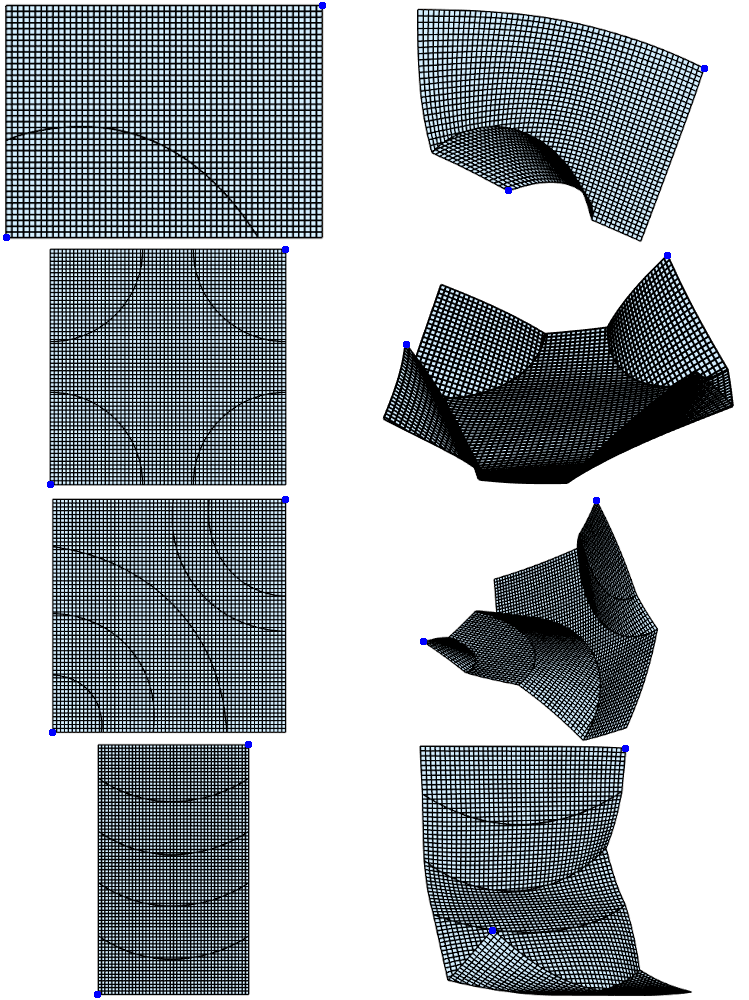
\includegraphics[width=0.99\linewidth]{../../../pics/0308_creasepatterns_results}
    \caption{Crease patterns: Flat initial state on the left, after bending on the right. From top to bottom: 1\_curve, 4\_corners, valley, parallel\_curves\_4}
    \label{fig:creasepatterns}
\end{figure}
The bulk of data presented in the following sections is gathered by performing the same operations on DOGs using different crease patterns, resolutions, and solver modes. The crease patterns are shown in figure \ref{fig:creasepatterns}. "1\_curve" is a very simple pattern with just one crease. "4\_corners" is also rather simple but includes more than two patches. "valley" and "parallel\_curves\_4" are more complicated and tend to be more problematic.\newline
\begin{table}
\centering
\begin{tabular}{|c|c|c|c|c|}
\hline
\multirow{2}{*}{crease pattern} & resolution $1$ & resolution $2$ & resolution $3$ & resolution $4$ \\ \cline{2-5}
 & \# vertices & \# vertices & \# vertices & \# vertices \\ \hline
 
\multirow{2}{*}{1\_curve} & $31 \times 21$ & $43 \times 31$ & $55 \times 41$ & $81 \times 59$ \\ \cline{2-5}
 & $721$ & $1435$ & $2389$ & $4969$ \\ \hline
\multirow{2}{*}{4\_corners} & $21 \times 21$ & $41 \times 41$ & $61 \times 61$ & $81 \times 81$ \\ \cline{2-5}
 & $569$ & $1937$ & $4105$ & $7073$ \\ \hline
\multirow{2}{*}{valley} & $21 \times 21$ & $41 \times 41$ & $61 \times 61$ & $81 \times 81$ \\ \cline{2-5}
 & $639$ & $2069$ & $4301$ & $7327$ \\ \hline
\multirow{2}{*}{parallel\_curves\_4} & $27 \times 45$ & $39 \times 65$ & $45 \times 75$ & $51 \times 85$ \\ \cline{2-5}
 & $1498$ & $2943$ & $3847$ & $4867$ \\ \hline
\end{tabular}
\caption{Mesh sizes for the test cases in figure \ref{fig:results_plotblock}}
\label{tab:res_and_vnum}
\end{table}
The resolutions used are tabulated in table \ref{tab:res_and_vnum}. The number of vertices is not just the product of $x$-resolution and $y$-resolution because the areas near creases are duplicated. Note how all resolutions are uneven: This ensures that the coarse DOG can be constructed correctly. Even resolutions would lead to an odd number of edges/quads in one direction, which makes it impossible to link the fine and coarse meshes correctly.\newline
The following solver modes are used: Standard (optimization on the global regular mesh), Coarse with no fine-to-coarse update (as described in chapter \ref{sec:coarse}), Coarse with fine-to-coarse update (with varying weights for the soft constraints on the link vertices). Other methods (like ADMM) were deemed unlikely to be an improvement over the standard solver and will not be considered here.\newline
Once the DOG is ready, we add positional constraints at two corners (marked by blue dots in figure \ref{fig:creasepatterns}). Over $250$ iterations the constraints are moved linearly towards a target position. Data is also gathered for $50$ iterations after that to see how the solver behaves once the constraints are fixed.\newline

\section{Test results}
\begin{figure}
    \centering
    \includegraphics[width=1\linewidth]{../../../pics/0308_plotblock}
    \caption{Objective function plotted over $300$ iterations for multiple crease patterns, resolutions, and solver modes. Starting from a flat initial state, the constraints reach their final state after $250$ iterations (marked by a dotted vertical line). Plots correspond to the crease patterns and resolutions in the same location in table \ref{tab:res_and_vnum}}
      \label{fig:results_plotblock}
\end{figure}
\begin{figure}
    \centering
    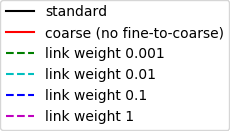
\includegraphics{../../../pics/0302_legend}
    \caption{Legend for figure \ref{fig:results_plotblock}}
    \label{fig:results_legend}
\end{figure}
Figure \ref{fig:results_plotblock} shows what happens with the objective functions. As can be seen, the standard and coarse solvers tend to have qualitatively similar results but the objective function always obtains lower values with the standard solver. That is because the standard solver optimizes the objective function directly while the coarse solver tries to do so using a different way. Interestingly, the coarse solver sometimes performs better without the fine-to-coarse update. It's still usually better to do the fine-to-coarse update (notice how the no-fine-to-coarse-update curve looks in the largest "1\_curve" setting in the upper right corner).\newline
The resulting meshes usually look very similar, whether the standard solver or the coarse solver is used (compare figure \ref{fig:results_compare_valley}). There are exceptions however: The crease pattern "parallel\_curves\_4" (seen in figure \ref{fig:results_compare_curves}) has quite different results: In the coarse solver the mesh ends up looking like a half-circle from the side, but in the standard solver all adjacent patches have very different orientations.\newline %TODO refer to fold bias
The coarse solver also has visibly different results for small meshes (i.e. the leftmost row). This happens because the coarse mesh still needs a certain size to work properly. In other words, making the resolution too low results in a coarse mesh that is too coarse to be useful.\newline
\begin{figure}
    \centering
    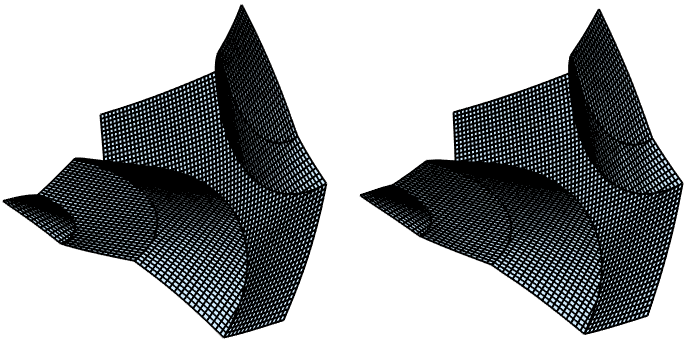
\includegraphics[width=0.8\linewidth]{../../../pics/0303_standard_vs_coarse_valley}
    \caption{Comparison between final state for crease pattern "valley" using standard solver (left) or coarse solver (right)}
      \label{fig:results_compare_valley}
\end{figure}
\begin{figure}
    \centering
    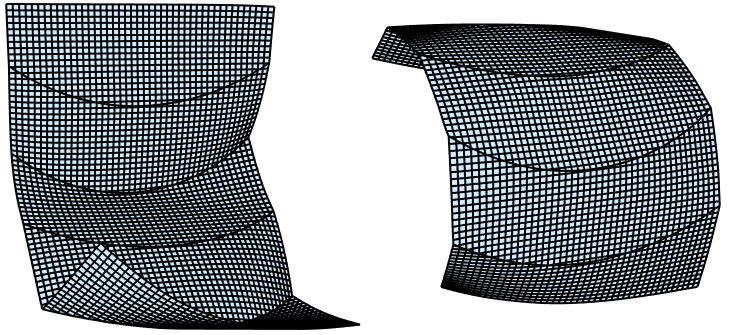
\includegraphics[width=0.8\linewidth]{../../../pics/0303_standard_vs_coarse_parallel_curves_4}
    \caption{Comparison between final state for crease pattern "parallel\_curves\_4" using standard solver (left) or coarse solver (right)}
      \label{fig:results_compare_curves}
\end{figure}
\section{Timing}
%coarse is faster ... but any patterns? not really
\begin{figure}
    \centering
    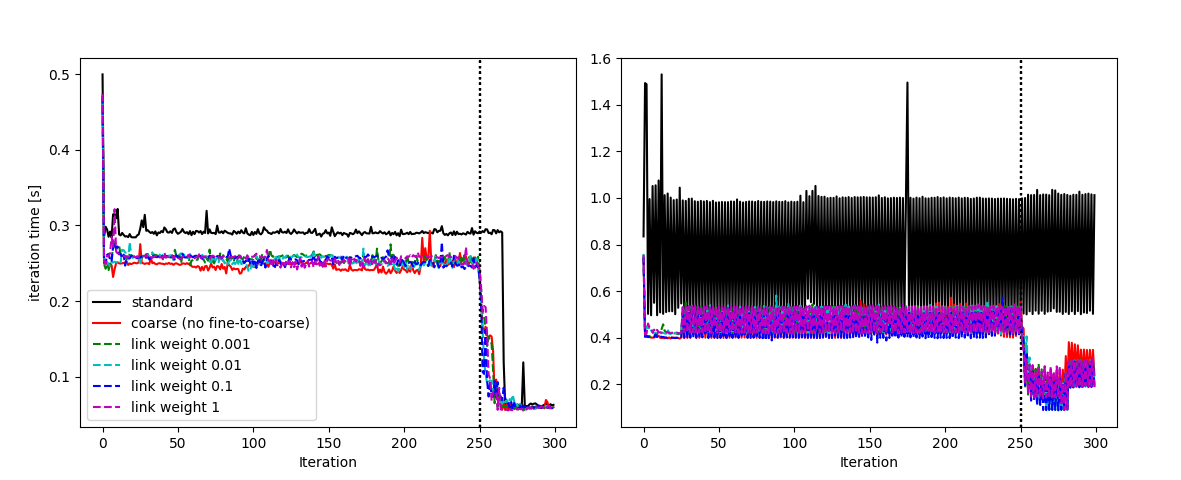
\includegraphics[width=0.99\linewidth]{../../../pics/0308_timeperiteration_examples}
    \caption{Time needed for iterations $1$ to $300$. Crease pattern "4\_corners" with resolution $41 \times 41$ on the left, crease pattern "parallel\_curves\_4" with resolution $39 \times 65$ on the right}
    \label{fig:results_cornerstime}
\end{figure}
\begin{figure}
    \centering
    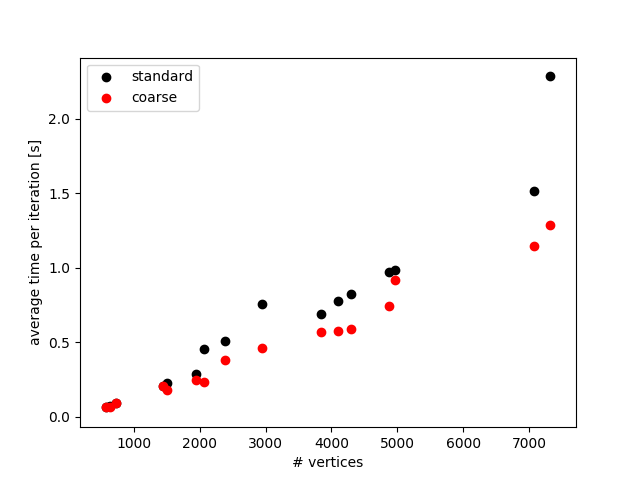
\includegraphics[width=0.7\linewidth]{../../../pics/0302_timeperiteration}
    \caption{Time per iteration, taken as the averaged in iterations $10$-$240$}
      \label{fig:results_timeperiteration}
\end{figure}
%also mention how the time varies between iterations, take averages, etc
The time per iteration, plotted over $300$ iterations, usually looks like the left example in figure \ref{fig:results_cornerstime}. The first iteration often takes more time than the later ones, then the time per iteration is roughly the same during the phase where te constraints are moving. Once the constraints arrive at their final positions, the solver usually finds a solution very quickly, after which there is nothing happening and the time per iteration is greatly decreased.\newline
The right side of figure \ref{fig:results_cornerstime} shows a more problematic example. About every second iteration in that case takes more time than the one before and after it. This happens because sometimes the solver needs to go back and redo the iteration with different parameters to enforce certain constraints (notice how the time the time for a standard iteration is either $0.5$ or $1$ second). It can also happen on the coarse mesh, but the difference in iteration time is less extreme there due to two factors: The coarse mesh is a smaller system than the global mesh, and the solver iterations on the fine patches also make up a major part of the work.\newline
Another thing that can be seen in the plot on the right is that sometimes the iterations don't become faster at the end. In fact, the time for later iterations can even be higher than for early iterations. This seems to happen only with the standard solver and not when using the coarse method.\newline
Following this, an average "time per iteration" is computed using iterations $10$ to $240$ and compared between solver mode and the number of vertices in figure \ref{fig:results_timeperiteration}. The time per iteration seems to scale linearly with the number of vertices and the coarse solver is consistently faster than standard for the same mesh size.\newline %TODO certain crease patterns profit more

%TODO parallelization gains (of course, there's no real data for that yet)
\chapter{Conclusion}\label{sec:conclusion}
%TODO
worth it? meh
\cite{dadada}% from "something"
\cite{athing}
%\cite{mal}
%\cite{Everitt2001OIT}% from "graphics"
%\cite{Schaufler00Ray}


%\clearpage
%\renewcommand*{\chapterpagestyle}{empty}

%TODO bibliography
%\cleardoublepage
%\phantomsection
\addcontentsline{toc}{chapter}{Bibliography}
\bibliography{sources}
%\bibliography{graphics}

\end{document}
